\section{Requerimientos de arquitectura}

\begin{enumerate}
  \item Base de datos 
  \begin{itemize}
    \item SQL Server 
        \begin{itemize}
            \item Microsoft SQL Server 2012 SP4 o superior o Microsoft Azure SQL Database Collation por defecto con el sufijo CS\_AS.
                
            \item El usuario de TIBCO EBX para conectarnos a la BS deberá tener los siguientes privilegios:
            \begin{itemize}
                \item CONNECT, SELECT and CREATE TABLE, en la base de datos que aloja el repositorio de TIBCO EBX. 
                \item ALTER, CONTROL, UPDATE, INSERT, DELETE, en el esquema.
            \end{itemize}
        \end{itemize}
  \end{itemize}
  \item Servidores
   \begin{itemize}
        \item Servidores QA y PRD.
    \end{itemize}

\end{enumerate}


\begin{figure}[H]
    \centering
    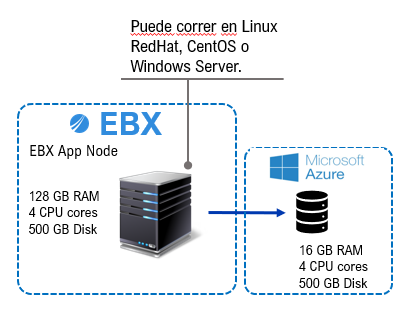
\includegraphics[width=0.4\textwidth]{Requerimientos/Arquitectura/ReqArquitectura.png}
    \caption{Requerimientos de Arquitectura.}
\end{figure}

\subsection{Links de descarga}
\textbf{TIBCO EBX:}

\href{https://edelivery.tibco.com/storefront/index.ep}{sitio oficial de TIBCO} Se requiere autenticación mediante usuario y contraseña. 

\href{https://tomcat.apache.org/tomcat-9.0-doc/index.html }{Descargar Tomcat}